% !TeX root = ../main.tex
\section{Ergebnisse}
\label{cap:ergebnisse}

Tabelle~\ref{tab:beispiel} zeigt eine Beispieltabelle im Stil der Bachelorarbeit.

\begin{table}[H]
	\centering
	\caption{Beispieltabelle mit an der Dezimalstelle ausgerichteten Zahlen}
	\label{tab:beispiel}
	\begin{tabular}{
			c
			S[table-format=1.3]
			S[table-format=2.2]
		}
		\toprule
		\textbf{Probe} & \textbf{Formparameter} & \textbf{Skalenparameter [\si{\newton}]} \\
		\midrule
		P1 & 5,849 & 38,27 \\
		P2 & 4,583 & 37,39 \\
		\bottomrule
	\end{tabular}
\end{table}

Abbildung~\ref{fig:vergleich} zeigt zwei Bilder nebeneinander.

\begin{figure}[H]
	\centering
	\begin{subfigure}{0.48\textwidth}
		\centering
		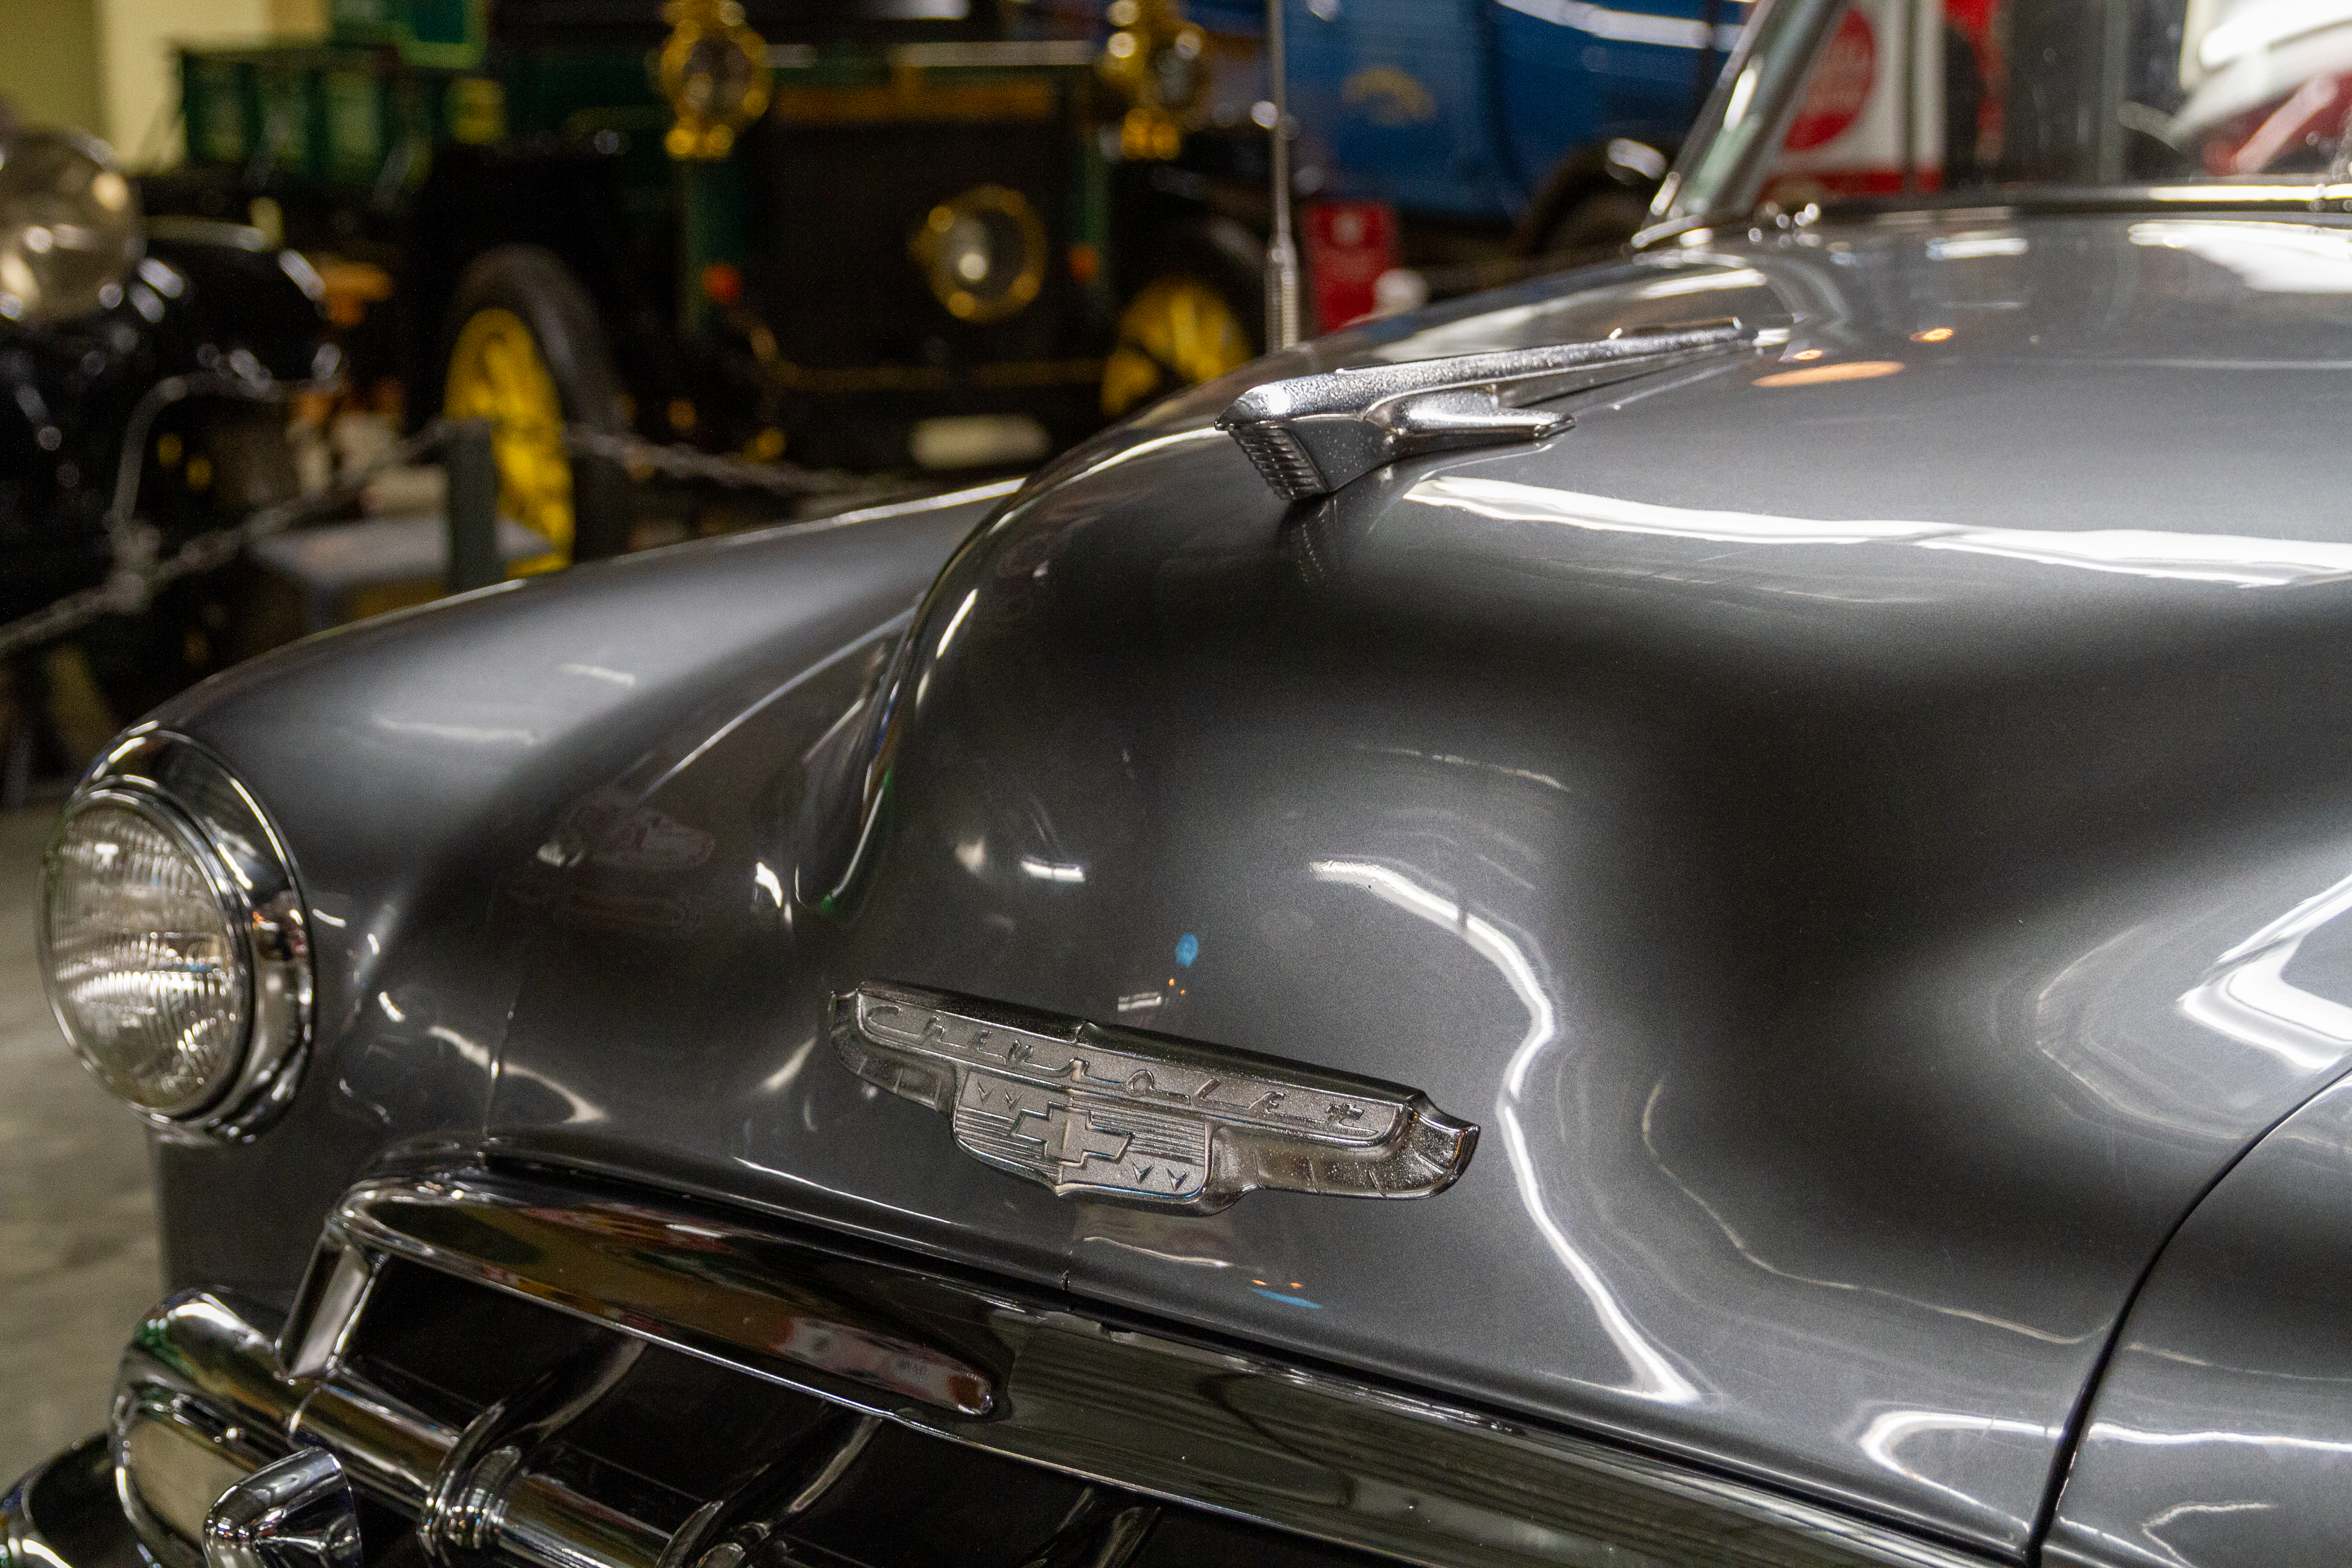
\includegraphics[width=\linewidth]{example-image-b}
		\caption{Variante A}
		\label{fig:vergleich_a}
	\end{subfigure}
	\hfill
	\begin{subfigure}{0.48\textwidth}
		\centering
		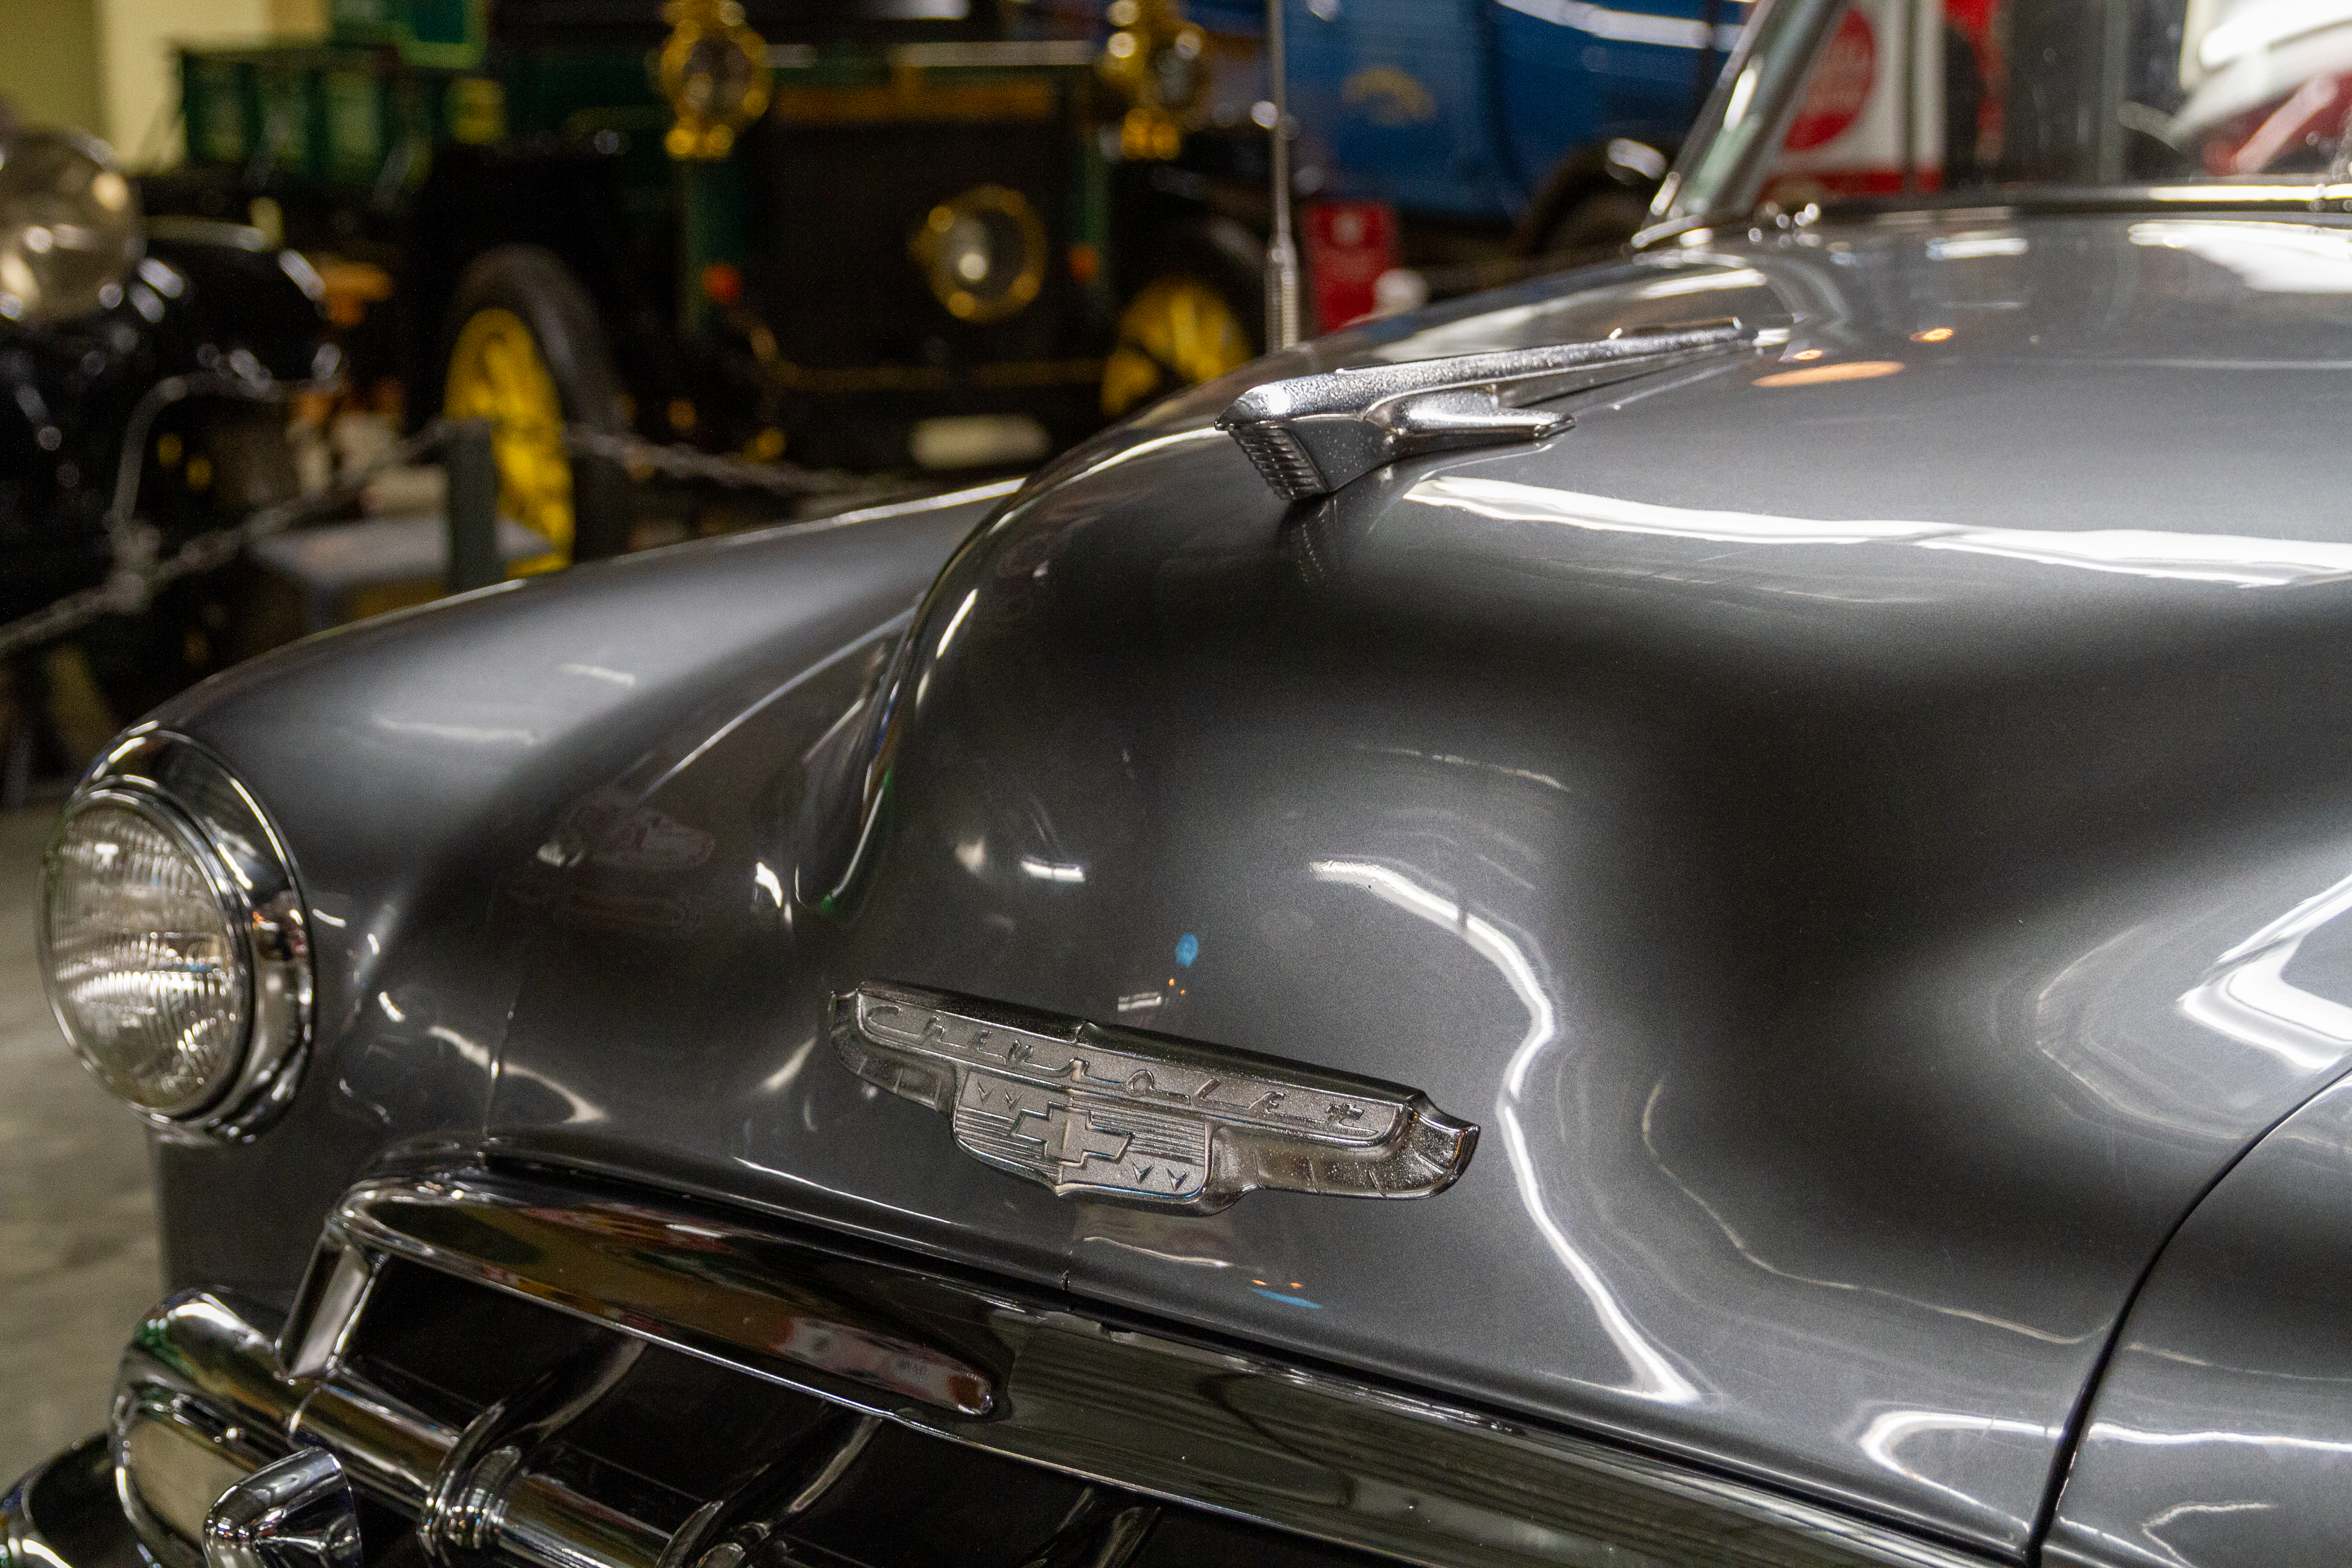
\includegraphics[width=\linewidth]{example-image-c}
		\caption{Variante B}
		\label{fig:vergleich_b}
	\end{subfigure}
	\caption{Vergleich zweier Varianten}
	\label{fig:vergleich}
\end{figure}
